\chapter{Stand der Technik}

Dieser Stand der Technik ordnet die Arbeit in den aktuellen Forschungsstand ein. Inhaltlich wird der zuerweiternde KI-gestützte Cutting Assistant beschrieben. Außerdem wird das 3D-Kantenmesssystem erläutert, mit dem die Trainingsdaten erfasst werden.

\section{KI-gestütztes Laserschneiden – Cutting Assistant}
\label{sec:cutting-assistent}

Der Cutting Assistant unterstützt die Qualitätssicherung und die Parametrierung beim Laserschneiden. Abbildung~\ref{fig:cutting_assistant} zeigt den Gesamtablauf von der Datenerfassung bis zur rückgekoppelten Optimierung der Prozessparameter. Zunächst erfasst einer am Schneidsystem montierter Handscanner die Schnittkante und übergibt die Bilddaten automatisiert an die Auswertekette. Ein vorgeschaltetes CNN (\enquote{Iron-hunter}, vgl. Abschnitt~\ref{sec:cnns}) prüft die Plausibilität der Aufnahme und verwirft Störbilder oder Fehlperspektiven. Beispiele für eine valide Kantenaufnahme und eine Fehlaufnahme sind in Abbildung~\ref{fig:ok-nok-examples} dargestellt. 

\begin{figure}[!htbp]
    \centering
    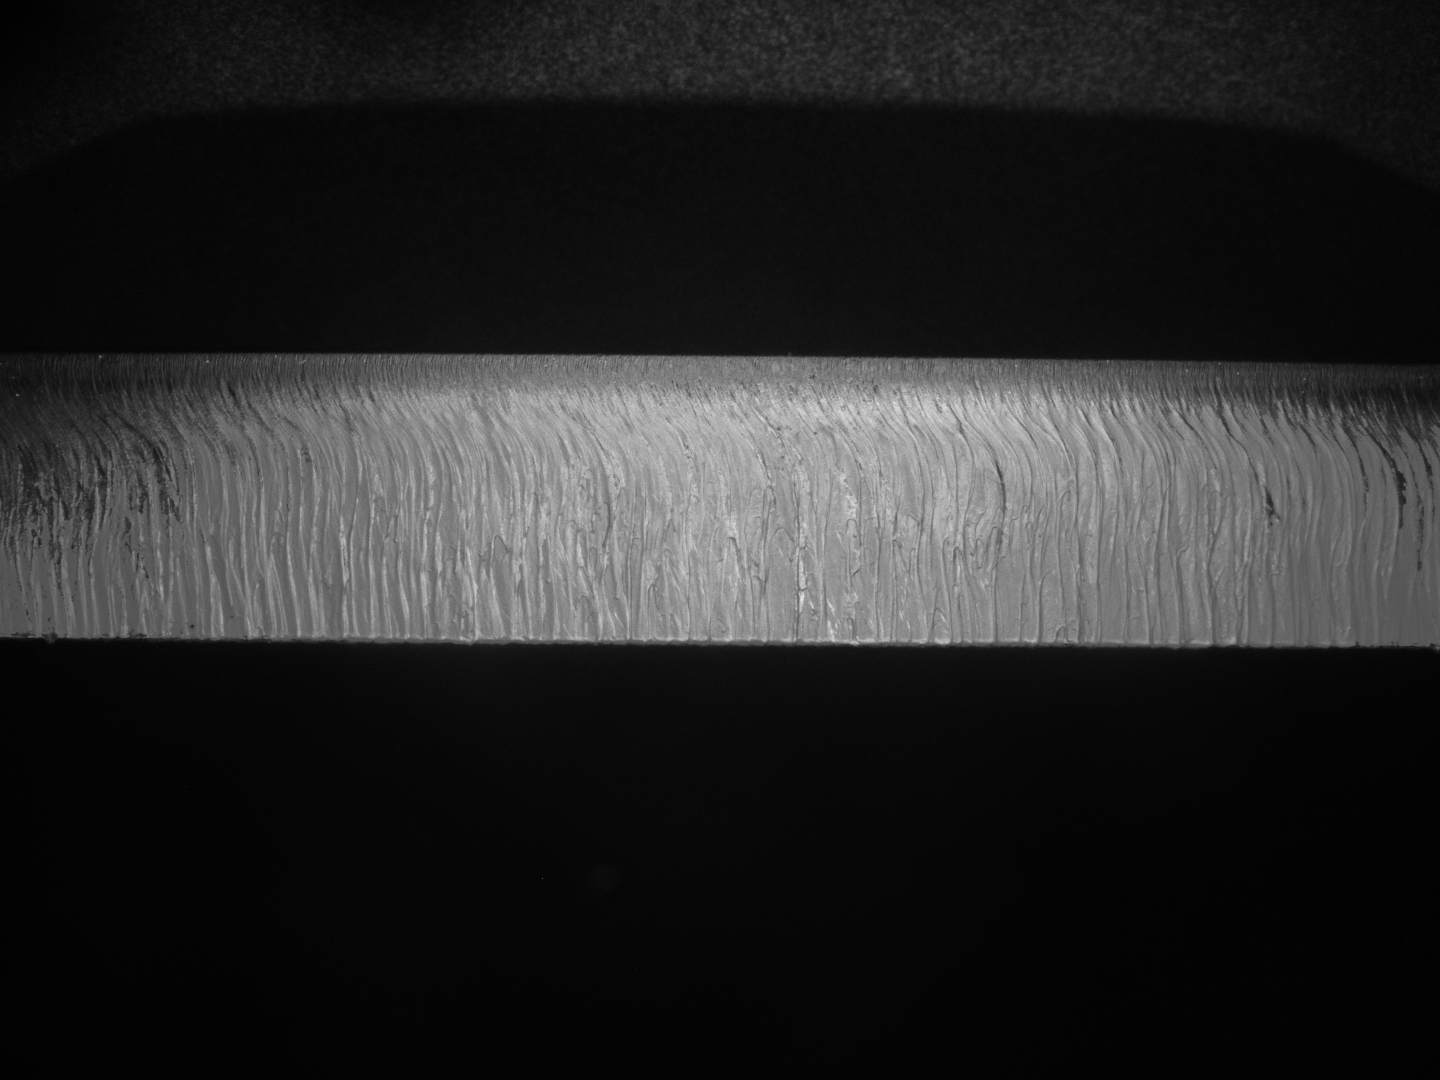
\includegraphics[width=0.49\linewidth]{valid_edge_image.png}\hfill
    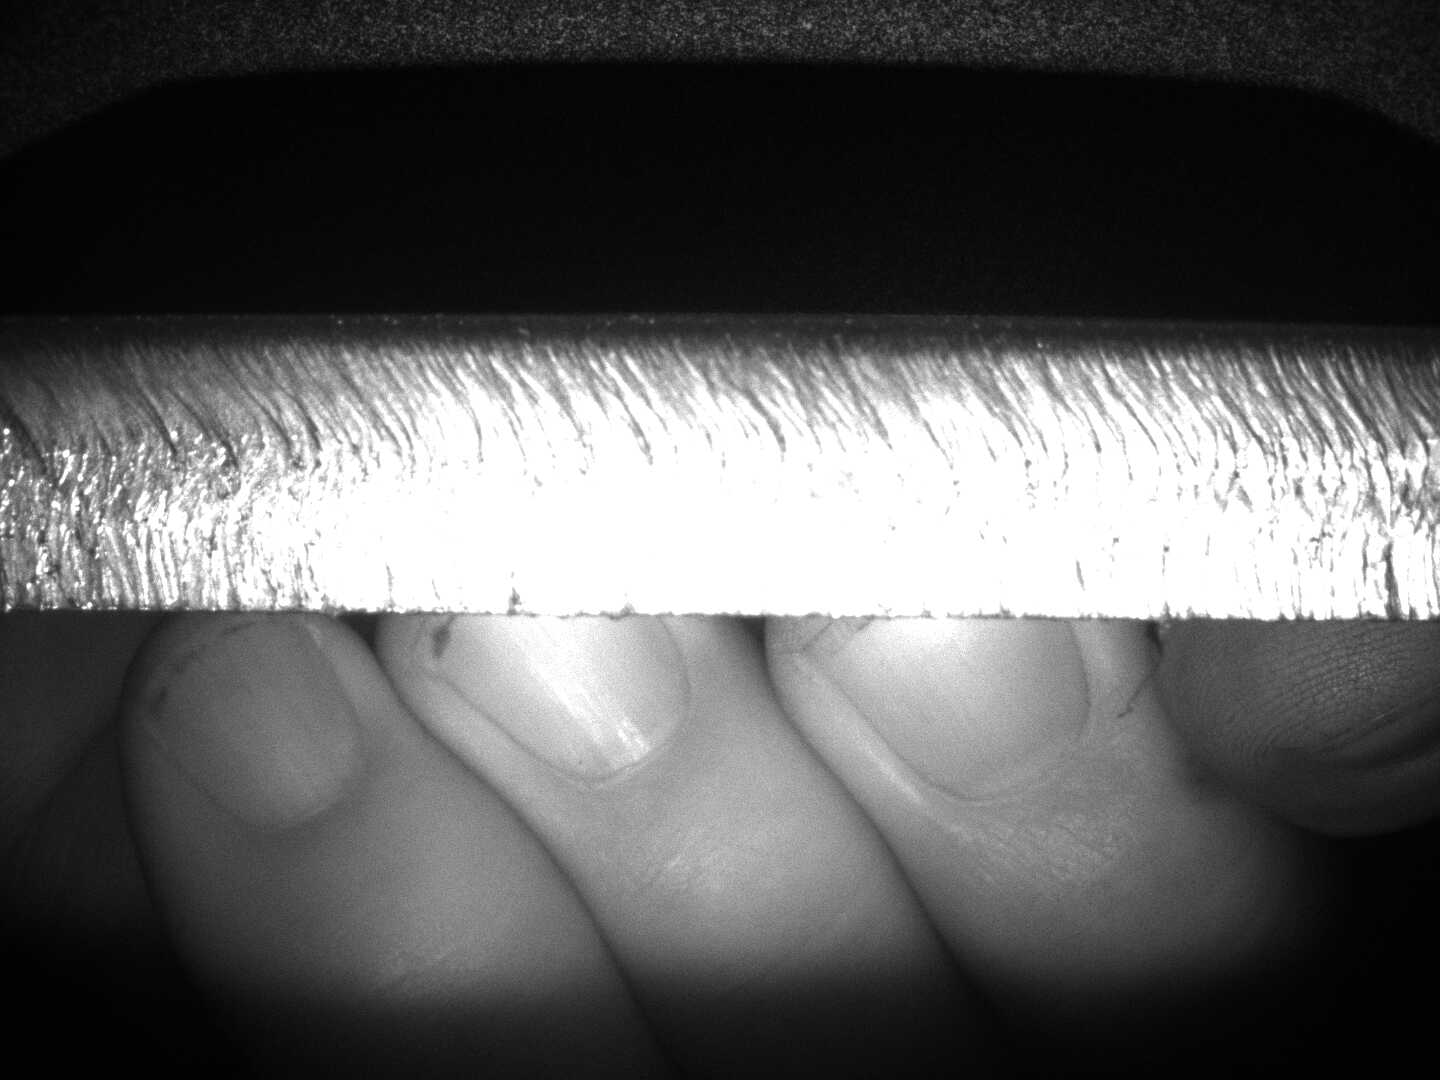
\includegraphics[width=0.49\linewidth]{finger_false_image.png}
    \caption{Beispiele zur Plausibilitätsprüfung durch \enquote{Iron-hunter}: links eine gültige Aufnahme der Schnittkante, rechts eine Fehlaufnahme mit verdeckender Hand, die verworfen wird.}
    \label{fig:ok-nok-examples}
\end{figure}

Nur valide Daten gelangen zur Detektion, wo ein zweites Netz eine Qualitätsschätzung durchführt und Merkmale wie Rauheit und Grat schätzt. Die Kennzahlen fließen in ein Optimierungsmodell ein, wobei Gasdruck, Fokuslage und Schneidgeschwindigkeit anpasst werden. Wie diese Schneidparameter die Schneidqualität beeinflussen wird im oben Grundlagenkapitel ~\ref{sec:laserlichtschneiden} näher erläutert.

Der Zyklus aus Aufnehmen, Bewerten und Anpassen wiederholt sich, bis ein Abbruchkriterium erfüllt ist, etwa wenn keine weitere Qualitätssteigerung zu erwarten ist oder die Spezifikation erreicht wurde. Das System ist für Baustahl validiert und wird im Rahmen dieser Arbeit auf Edelstahl erweitert, indem Datensätze ergänzt, Netzparameter feinjustiert und Schwellwerte an das Werkstoffverhalten angepasst werden.

\begin{figure}[!htbp]
    \centering
    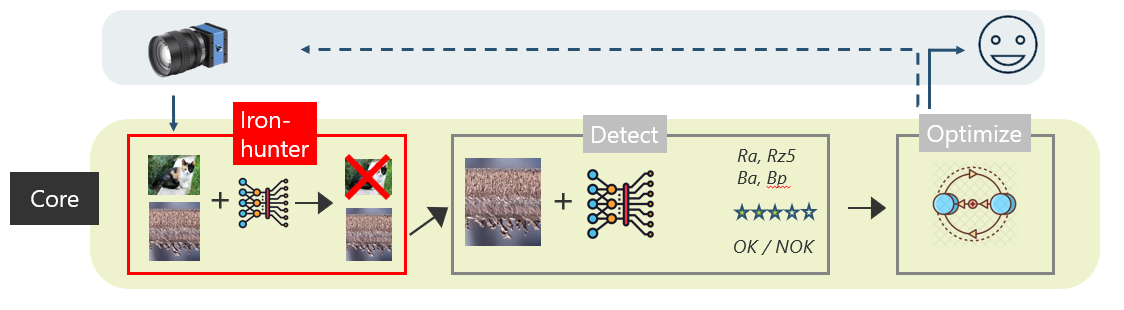
\includegraphics[width=0.95\linewidth]{cutting_assistant_pipeline.png}
    \caption{Prozesskette des Cutting Assistant.}
    \label{fig:cutting_assistant}
\end{figure}



\section{3D-Kantenmesssystem: Keyence LJ-X8060}
\label{sec:3d-messsystem-keyence}

In diesem Abschnitt wird die Funktionsweise des bereits eingesetzten dreidimensionalen Messsystems beschrieben, mit dem die Schnittkanten der Trainingsdaten für das KI-Modell erfasst wurden. Das System wurde zunächst für das Baustahlmodell verwendet und wird für die vorliegende Arbeit auf die Vermessung von Edelstahl angepasst. Die dafür notwendigen Optimierungen sind in Kapitel~\ref{chap:3d-punktwolken-optimierung} beschrieben.

Abbildung~\ref{fig:lasertriangulation-schema} zeigt den Aufbau eines Sensors auf Basis der Lasertriangulation. Eine Sendeoptik projiziert eine Laserlinie auf die Oberfläche des Werkstücks. Versetzt zur Sendeeinheit erfasst eine Empfangsoptik das reflektierte Licht und bildet es auf einen zeilenförmigen Detektor ab. Die Position der Lichtlinie auf dem Detektor hängt von der Objektentfernung ab. Aus dieser Geometrie wird für jedes Zeilenprofil die Höhe des zugehörigen Oberflächenpunkts berechnet. Durch die Relativbewegung zwischen Sensor und Objekt entstehen aufeinanderfolgende Profile, die zu einer dreidimensionalen Punktewolke mit \((x,y,z)\) zusammengeführt werden.

\begin{figure}[h!]
    \centering
    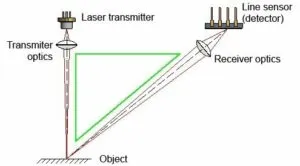
\includegraphics[width=0.4\linewidth]{keyence_triangulation.png}
    \caption{Lasertriangulation zur Profilaufnahme.}
    \label{fig:lasertriangulation-schema}
\end{figure}

Abbildung~\ref{fig:schnittkante-setup} fasst die Erfassung mit dem Keyence LJ-X8060 zusammen. Links ist der schematische Messaufbau mit Koordinatensystem gezeigt. Die Laserlinie tastet die Kante quer zur Scanrichtung ab und die Bewegung erfolgt entlang \(x\). Rechts ist eine registrierte dreidimensionale Punktewolke im Werkstückkoordinatensystem \((x,y,z)\) dargestellt. Für die Auswertung werden die Daten durch eine Koordinatenrotation so ausgerichtet, dass die Kante mit der \(x\)-Achse und die Blechebene mit der \(xy\)-Ebene zusammenfällt.

\begin{figure}[h!]
    \centering
    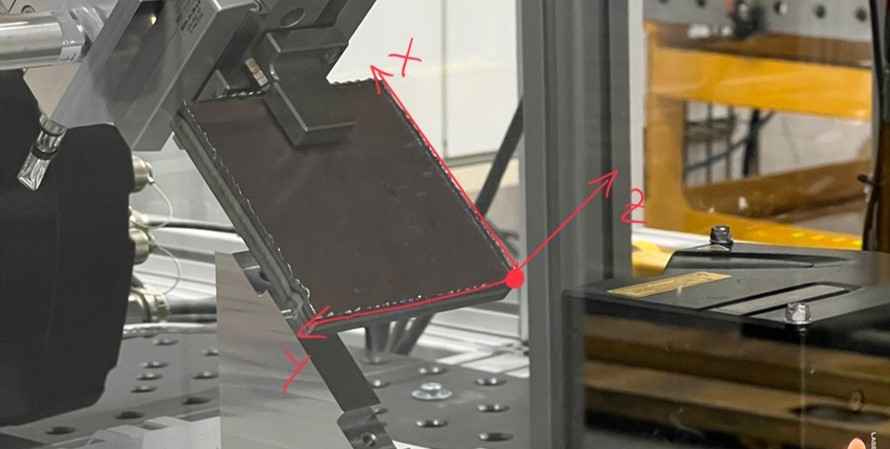
\includegraphics[width=0.49\linewidth]{baustahlmessung_keyence.png}\hfill
    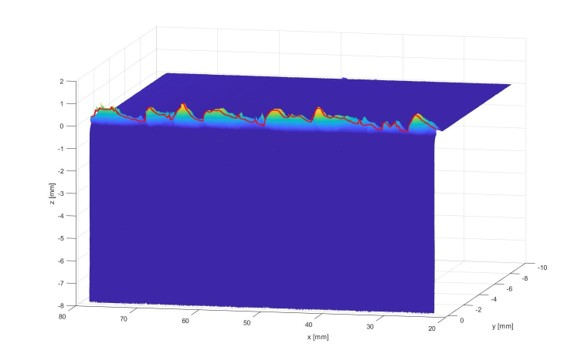
\includegraphics[width=0.49\linewidth]{3D-Punktewolke.jpg}
    \caption{Messaufbau und Beispielpunktwolke der Schnittkante für den Gratverlauf.}
    \label{fig:schnittkante-setup}
\end{figure}

Aus der erfassten dreidimensionalen Punktewolke wird ein zweidimensionaler Vektor abgeleitet, der den Gratverlauf im \(yz\)-Schnitt beschreibt. Da die Schnittkante schräg erfasst wird, richtet eine Koordinatenrotation die Profile auf das Werkstückkoordinatensystem aus. Die Kante fällt danach mit der \(x\)-Achse zusammen und die Blechebene mit der \(xy\)-Ebene. Die Rauheit der Schnittfläche wird als zweidimensionaler Vektor in der \(xy\)-Ebene beschrieben. Die Auswertung erfolgt entlang \(x\) und wird über \(y\) gemittelt. Eine ausführliche Beschreibung der Berechnung von Grat und Rauheit ist in Abschnitt~\ref{sec:grat-rauheit} zu finden.
